\begin{table}[h]
    \centering
    \caption{Сравнение характеристик шаблонизаторов}
    \begin{tabular}{|l|c|c|c|c|}
        \hline
        \textbf{Характеристика} & \textbf{MLX} & \textbf{TyXML} & \textbf{Dream HTML} & \textbf{Dream EML}               \\
        \hline
        Типобезопасность        & \checkmark   & \checkmark     & \texttimes          & \texttimes                       \\
        Чистота функций         & \texttimes   & \checkmark     & \checkmark          & \colorbox{orange!30}{\checkmark} \\
        Произвольные строки     & \texttimes   & \texttimes     & \checkmark          & \colorbox{orange!30}{\checkmark} \\
        Вес (KB)                & 142          & 89             & 63                  & \colorbox{orange!30}{27}         \\
        \hline
    \end{tabular}
\end{table}

\textbf{Преимущества Dream EML}:
\begin{itemize}
    \item Нативная интеграция с Dream
    \item Минимальная зависимость от внешних библиотек
    \item Поддержка inline-выражений OCaml
    \item HTML-подобный синтаксис
\end{itemize}


\begin{table}[h]
    \centering
    \caption{Сравнение времени рендеринга (в секундах) для разных шаблонизаторов}
    \label{tab:rendering-times}
    \begin{tabular}{lrrrr}
        \toprule
        \textbf{Шаблонизатор} & \textbf{100} & \textbf{1000} & \textbf{10,000} & \textbf{100,000} \\
        \midrule
        MLX                   & 0.000117     & 0.000969      & 0.015393        & 0.139218         \\
        TyXML                 & 0.000423     & 0.003726      & 0.026868        & 0.241985         \\
        TyXML\%               & 0.000508     & 0.004809      & 0.033487        & 0.236966         \\
        Dream html            & 0.000041     & 0.001579      & 0.003616        & 0.034738         \\
        Dream eml             & 0.001917     & 0.005415      & 0.040749        & 0.281302         \\
        \bottomrule
    \end{tabular}
\end{table}

% // TODO: доделать график, чтоыб он включал в себя бОльшие величины, а также просто больше величин. Возможно, выделить какие-то особенности других фреймворков.

\begin{figure}
    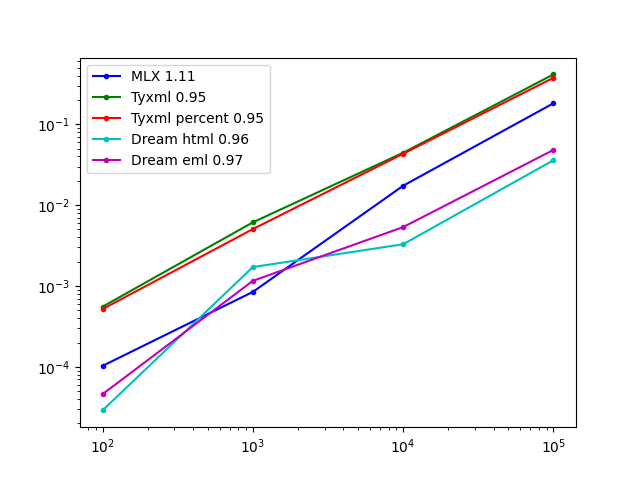
\includegraphics[width=\textwidth]{perfomance.png}
    \label{fig:perfomance}
    \caption{Сравнение производительности шаблонизаторов. График построен с помощью пакета matplotlib. Числа в легенде соответствуют аппроксиммированному углу наклона прямых. Масштаб выбран логарифмическим}
\end{figure}

График построен используя matplotlib python.

Анализ графика:

\begin{table}[h]
    \centering
    \caption{Сравнение характеристик шаблонизаторов}
    \label{tab:templates-comparison}
    \begin{tabular}{lp{3cm}p{3cm}p{2cm}p{3cm}p{2cm}}
        \toprule
        \textbf{Характеристика}                        & \textbf{eml} & \textbf{mlx} & \textbf{TyXML} & \textbf{TyXML let\%html} & \textbf{dream-html} \\
        \midrule
        Сохранение синтаксиса                          &
        Нет, преобразуется во внутреннее представление &
        Нет, преобразуется в OCaml                     &
        Да                                             &
        Да                                             &
        Да                                                                                                                                             \\

        Читаемость                                     &
        Нет, внутреннее представление сжато            &
        Да, результирующий OCaml читаем                &
        Да                                             &
        Да                                             &
        Да                                                                                                                                             \\

        Комментарии                                    &
        ---                                            &
        ---                                            &
        ---                                            &
        Только OCaml-части покрыты                     &
        ---                                                                                                                                            \\
        \bottomrule
    \end{tabular}
\end{table}